\section{ОР-матрицы и усиленные ОР-матрицы}

\begin{definition}
  \textbf{Однозначно разрешимой матрицей} (сокр. ОР-матрицей, англ. uniquely solvable puzzle, USP) ширины $k$ называют подмножество $U \subseteq \left\{ 1,2,3 \right\}^k$, удовлетворяющее свойству: 
  
  для любой тройки перестановок $\pi_1, \pi_2, \pi_3 \in S_U$ либо $\pi_1=\pi_2=\pi_3$, либо существуют $u \in U$ и $i \in [k]$ такие, что по меньшей мере два равенства из 
  \[\left( \pi_1(u) \right)_i = 1,\; \left( \pi_2(u) \right)_i = 2,\; \left( \pi_3(u) \right)_i = 3\]
  выполняются. (Здесь $\left( \pi_j(u) \right)_i$ обозначает число, стоящее на $i$-ой позиции в строке $\pi_j(u)$.)
\end{definition}

В качестве примера ОР-матрицы ширины 6 и размера 8 можно привести следующую таблицу:
\begin{figure}[H]
	\begin{center}
	   \begin{tabular}{|c|c|c|c|c|c|}
	    \hline 
	    3 & 3 & 3 & 3 & 3 & 3\\ \hline
	    1 & 3 & 3 & 2 & 3 & 3\\ \hline
	    3 & 1 & 3 & 3 & 2 & 3\\ \hline
	    1 & 1 & 3 & 2 & 2 & 3\\ \hline
	    3 & 3 & 1 & 3 & 3 & 2\\ \hline
	    1 & 3 & 1 & 2 & 3 & 2\\ \hline
	    3 & 1 & 1 & 3 & 2 & 2\\ \hline
	    1 & 1 & 1 & 2 & 2 & 2\\ 
	    \hline
	  \end{tabular}
	\end{center}
	\caption{Пример ОР-матрицы}
	\label{usp}
\end{figure}
Замечу, что порядок, в котором следуют строки, значения не имеет. 

В английском наименовании этого объекта присутствует слово пазл, потому что ОР-матрицу можно рассматривать как своего рода головоломку. Пусть 
\[
u = \begin{array}{|c|c|c|c|c|c|} \hline 3 & 3 & 1 & 3 & 3 & 2 \\ \hline\end{array} 
\]
--- это один из элементов $U$. Он состоит из частей трёх типов
\[
	\begin{array}{|c|c|c|c|c|c|} \hline \; & \; & 1 & \; & \; & \;  \\ \hline\end{array}, 
	\begin{array}{|c|c|c|c|c|c|} \hline \; & \; & \;& \; & \; & 2 \\ \hline\end{array},
	\begin{array}{|c|c|c|c|c|c|} \hline 3 & 3 & \; & 3 & 3 & \; \\ \hline\end{array}.
\]
Чтобы собрать пазл, нужно переместить фрагменты первого, второго и третьего типов всех элементов $U$ в соответствии с перестановками $\pi_1, \pi_2, \pi_3$, и снова объединить их в таблицу так, чтобы в каждой строке новой матрицы были части каждого из трёх типов, и чтобы эти части не накладывались друг на друга. Определение требует, чтобы этот пазл имел единственное решение. То есть если среди перестановок $\pi_1, \pi_2, \pi_3$ будет по крайней мере две не равные между собой, то случится коллизия, то есть наложение частей. Если же все перестановки равны, то полученная в итоге матрица будет отличаться от исходной лишь порядком следования строк, что считается тем же самым решением.

Теперь немного подробнее. Сначала замечу, что для перестановок $\pi_1, \pi_2, \pi_3$ значение имеют только элементы 1,2 и 3 соответственно, стоящие в матрице. Поэтому лучше думать об этих перестановках не как о перемещающих строки целиком, а как о перемещающих фрагменты строк, содержащие их собственные числа. В этой интерпретации ОР-матрица с рисунка \ref{usp} будет выглядеть как:

\begin{figure}[H]
	\centering
    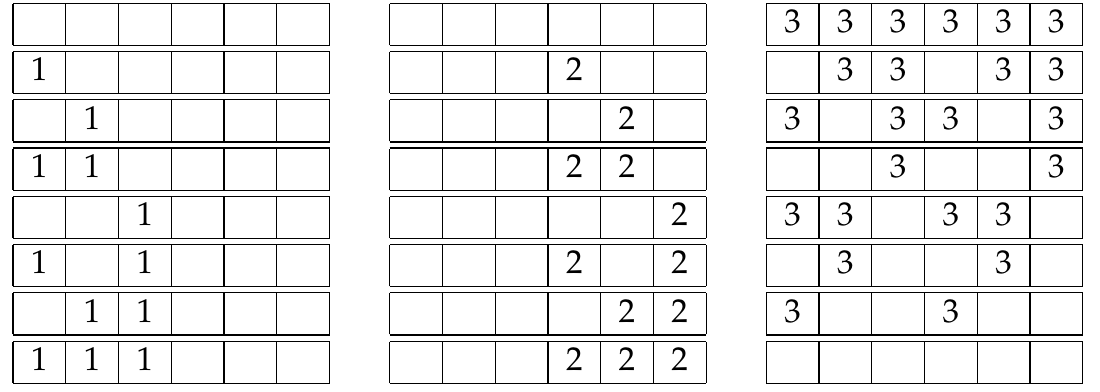
\includegraphics[width=0.5\textwidth]{figures/usp_pieces}
	\caption{фрагменты ОР-матрицы}
	\label{usp:fig3.2}
\end{figure}
Здесь в первую таблицу попадают все вхождения 1 в ОР-матрицу, во вторую --- 2, в третью --- 3. Далее $\pi_j$ перемещает строки таблицы, в которой стоят одни только $j$. В конце эти таблицы совмещаются. Равенство $(\pi_j(u))_i = j$ эквивалентно тому, что в итоговой таблице на пересечении строки $\pi_j(u)$ и столбца $i$ стоит число $j$. Поэтому из определения ОР-матрицы будет следовать, что если не все $\pi_j$ равны, то в итоговой таблице существует строка и столбец, на пересечении которых стоит больше одного элемента, то есть случилась коллизия, иначе говоря фрагменты пазла наложились друг на друга. 

Используя эту интерпретацию, докажем, что таблица с рисунка \ref{usp} на самом деле является ОР-матрицей. Без ограничения общности можно считать, что $\pi_3 = 1$ потому, что перебор всех троек $\pi_1, \pi_2, \pi_3$ эквивалентен перебору троек $\pi_1 \rho, \pi_2 \rho, \pi_3 \rho$ для какого-то $\rho \in S_U$. Выберем $\rho = \pi_3^{-1}$, в этом случае $\pi_1 \rho, \pi_2 \rho$ по-прежнему случайные перестановки, хотя $\pi_3 \rho$ теперь всегда равна 1. Это даст нам начальную позицию, изображённую ниже:
\begin{figure}[H]
	\centering
    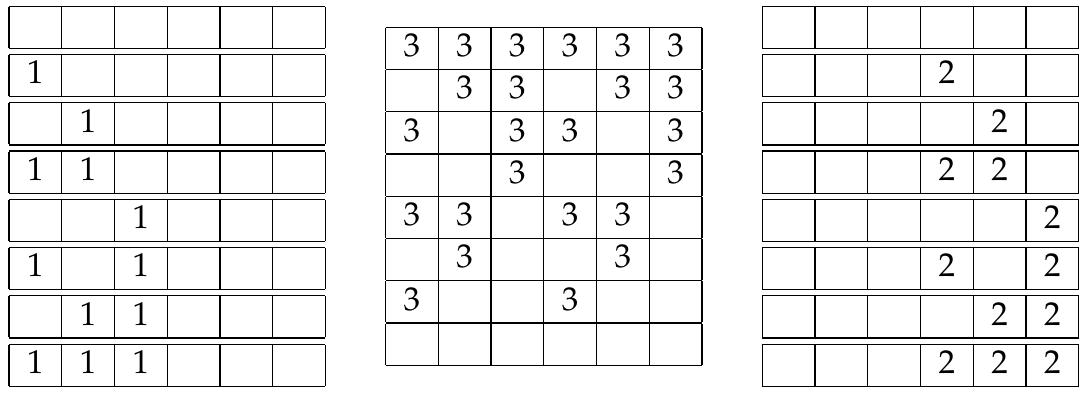
\includegraphics[width=0.5\textwidth]{figures/usp_threes_placed}
	\caption{фрагменты ОР-матрицы, где тройки уже на месте}
	\label{usp:fig3.3}
\end{figure}
Таблица в центре --- это пока ещё не завершённая итоговая таблица, оставшиеся части пазла изображены справа и слева. Так как $\pi_3 = 1$, мы знаем, что тройки уже стоят на своих местах.

Рассмотрим то, как будет выбираться место для фрагмента с тремя 1. Поскольку все строки, кроме последней, содержат 3 в одном из первых трёх столбцов, то попытка вставить этот фрагмент куда-либо помимо последней строки приведёт к коллизии. После того как фрагмент с тремя 1 займёт своё место пазл будет выглядеть так:
\begin{figure}[H]
	\centering
    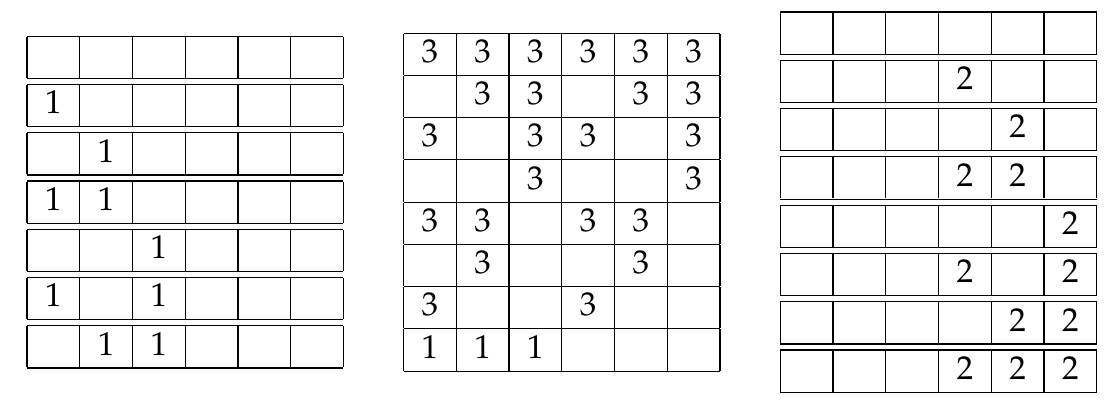
\includegraphics[width=0.5\textwidth]{figures/usp_threes_and_first_piece_placed}
	\caption{фрагменты ОР-матрицы, где тройки и фрагмент с тремя 1 уже на месте}
	\label{usp:fig3.4}
\end{figure}

Теперь рассматривая любой фрагмент с двумя 1, снова убеждаемся, что существует только одно место, куда его можно вставить без коллизий. Подобным же образом размещаются части с одной 1. В итоге получим:
\begin{figure}[H]
	\centering
    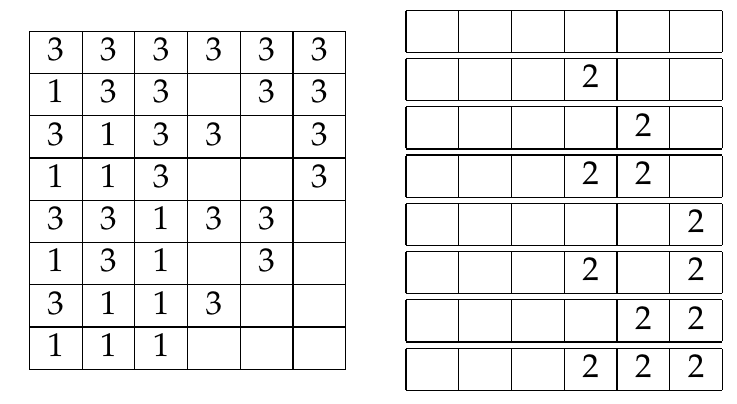
\includegraphics[width=0.5\textwidth]{figures/usp_threes_and_ones_placed.png}
	\caption{фрагменты ОР-матрицы, где тройки и единицы уже на месте}
	\label{usp:fig3.5}
\end{figure}

Так как структура фрагментов с двойками та же самая что и у фрагментов с единицами просто в других столбцах, ясно что они могут быть расположены единственным способом. Таким образом, показали, что матрица с рисунка \ref{usp} имеет единственное решение и поэтому на самом деле будет ОР-матрицей.

Нужно сделать одно дополнительное замечание о том случае, когда у таблицы, претендующей на звание ОР-матрицы, два фрагмента или строки идентичны, то есть имеют одни и те же числа и конфигурацию. В этом случае можно взять перестановку, которая будет просто менять эти две строки местами, что не будет менять саму матрицу, а две другие перестановки взять тривиальными. Тогда итоговая таблица будет идентична изначальной, то есть коллизий не будет, но также не будет выполняться условие $\pi_1=\pi_2=\pi_3$. Поэтому такая матрица не может быть однозначно разрешимой. Эта ситуация похожа на ту, когда в пазле есть два совершенно неотличимых фрагмента, и, конечно же, такой пазл не будет иметь единственного решения.

\begin{definition}
  \textbf{Усиленной ОР-матрицей} (сокр. УОР-матрицей) называют ОР-матрицу, у которой определяющее свойство было усилено следующим образом:
  
  для любой тройки перестановок $\pi_1, \pi_2, \pi_3 \in S_U$ либо $\pi_1=\pi_2=\pi_3$, либо существуют $u \in U$ и $i \in [k]$ такие, что \textbf{в точности} два равенства из 
  \[\left( \pi_1(u) \right)_i = 1,\; \left( \pi_2(u) \right)_i = 2,\; \left( \pi_3(u) \right)_i = 3\]
  выполняются.
\end{definition}

Возвращаясь к аналогии с пазлом, это условие означает, что теперь если в каких-то позициях произойдёт одновременное наложение сразу трёх фрагментов, это не будет нарушением правил сборки головоломки, то есть гораздо меньше матриц будет иметь единственное решение, поэтому это условие будет сильнее чем исходное.

Нетрудно заметить, что матрица с рисунка \ref{usp} будет УОР-матрицей, поскольку в каждом её столбце встречаются только два из возможных трёх символов $\left\{ 1,2,3 \right\}$. Эту конструкцию можно обобщить.

\begin{prop}\label{prop:05:3.1}
  Для любого $k \geq 1$ существует УОР-матрица размера $2^k$ и ширины $2k$.
\end{prop}
\begin{proof}
	Если смотреть на $\left\{ 1,3 \right\}^k \times \left\{ 2,3 \right\}^k$ как на подмножество $\left\{ 1,2,3 \right\}^{2k}$, определим $U$ следующим образом:
	\[
		\left\{ u \in \left\{ 1,3 \right\}^k \times \left\{ 2,3 \right\}^k | \text{ для } i \in [k], \; u_i = 1 \iff u_{i+k} = 2 \right\}.
	\]
	Пусть $\pi_1, \pi_2, \pi_3 \in S_U$. Если $\pi_1 \neq \pi_3$, тогда существует $u \in U$ такой, что $\left( \pi_1(u) \right)_i = 1$ и $\left( \pi_3(u) \right)_i = 3$ для
	какого-то $i \in [k]$. Точно также, если $\pi_2 \neq \pi_3$, тогда существует $u \in U$ такой, что $\left( \pi_2(u) \right)_i = 2$ и $\left( \pi_3(u) \right)_i = 3$ для
	какого-то $i \in [2k]\setminus[k]$. В любом случае в точности два равенства из $\left( \pi_1(u) \right)_i = 1,\; \left( \pi_2(u) \right)_i = 2,\; \left( \pi_3(u) \right)_i = 3$ выполняются, потому что в каждой координате могут встретиться только два из трёх символов $\left\{ 1,2,3 \right\}$. Отсюда следует, что $U$ является УОР-матрицей. 
\end{proof}

\begin{definition}
  \textbf{УОР-ёмкостью} называют наибольшую константу $C$ такую, что существуют УОР-матрицы размера $(C - o(1))^k$ и ширины $k$ для бесконечного количества значений $k$. \textbf{ОР-ёмкость} определяется аналогично.
\end{definition}

Существует простая верхняя оценка для ОР-ёмкости, которая, конечно, также будет верхней оценкой для УОР-ёмкости:
\begin{lemma} \label{lem:05:3.2}
  ОР-ёмкость не превышает ${3 \over 2^{2 / 3}}$.
\end{lemma}
\begin{proof}
  Пусть $U$ --- ОР-матрица ширины $k$. Для каждой тройки $n_1, \; n_2, \; n_3$ неотрицательных целых чисел, дающих в сумме $k$, определим $U_{u_1,u_2,u_3}$ как подмножество элементов $U$, которые имеют $n_1$ позицию с 1, $n_2$ позиций с 2, и $n_3$ с 3. Существует всего $\binom{k+2}{2}$ способов выбрать $n_1, n_2$ и $n_3$ поэтому
  \[
  	|U| \leq \dbinom{k+2}{2} \max_{n_1,n_2,n_3} |U_{n_1,n_2,n_3}|.
  \]
  Если два элемента $U$ имеют 1 в одних и тех же позициях, то если взять в качестве $\pi_1$ перестановку, которая меняет местами эти элементы, а $\pi_2, \pi_3$ взять тривиальными, то получим противоречие с определением ОР-матрицы, поэтому $|U_{n_1,n_2,n_3}|$ не может превосходить число способов, которым можно распределить $n_1$ единицу по имеющимся $k$ позициям, конечно, тоже самое будет верно для 2 и 3. Таким образом,
  \[
  	|U_{n_1,n_2,n_3}| \leq \min_i \dbinom{k}{n_i} \leq \left( {3 \over 2^{2/3}} + o(1)\right)^k,
  \]
  где последнее неравенство выполняется потому, что $\min_i \binom{k}{n_i}$ максимально, когда $n_1=n_2=n_3=k/3$. 
  
  \begin{align*}
    \ln \dbinom{k}{k/3} & = \ln \frac{k!}{(\frac{2k}{3})!(\frac{k}{3})!}\\
    & = \ln k! - \ln \left( \frac{2k}{3} \right)! - \ln \left( \frac{k}{3} \right)! \\
    & = k \ln k - \cancel{k} - \frac{2k}{3} \ln \frac{2k}{3} + \cancel{\frac{2k}{3}} - \frac{k}{3} \ln \frac{k}{3} + \cancel{\frac{k}{3}} + O(\ln k) \text{ (по формуле Стирлинга) }\\
    & = k \left( \ln k - \frac{2}{3} \ln \frac{2k}{3} - \frac{1}{3} \ln \frac{k}{3} \right) + O(\ln k)\\
    & = k \left( \cancel{\ln k} - \cancel{\frac{2}{3} \ln k} - \frac{2}{3} \ln \frac{2}{3} - \cancel{\frac{1}{3} \ln k} - \frac{1}{3} \ln \frac{1}{3} \right) + O(\ln k) \\
    & = k \left( - \frac{2}{3} \ln 2 + \frac{2}{3} \ln 3 + \frac{1}{3} \ln 3 \right) + O(\ln k)\\
    & = k \ln \frac{3}{2^{2/3}} + O(\ln k)\\
    & = k \left( \ln \left( \frac{3}{2^{2/3}} + o(1) \right) \right)
  \end{align*}
  \begin{question}
    Правильно ли я внёс $O(\ln k) / k$ в логарифм с получением в итоге $o(1)$?
  \end{question}
  Отсюда следует, что $|U| \leq \left( {3 \over 2^{2/3}} + o(1)\right)^k$, что и требовалось доказать.
\end{proof}

ОР-матрицы неявно присутствуют в статье Копперсмита и Винограда \cite{Coppersmith:1990}. Раздел 6 их статьи можно интерпретировать как вероятностную конструкцию, показывающую, что лемма \ref{lem:05:3.2} точная.

\begin{theorem} (Копперсмит и Виноград \cite{Coppersmith:1990}) \label{th:05:3.3}
  ОР-ёмкость равна ${3 \over 2^{2 / 3}}$.
\end{theorem}

Кон и др. в статье \cite{Cohn05} выдвинули гипотезу, что тоже будет верно для УОР-ёмкости. Если их гипотеза верна, то это будет означать, что $\omega=2$.
\begin{conj} \label{conj:05:3.4}
  УОР-ёмкость равна ${3 \over 2^{2 / 3}}$.
\end{conj}














